\documentclass[11pt]{article}
%%% Preamble for Pomona Linguistics Paper Template %%%

%%%%%%%%%%%%%%%%%%%%%%%%%%%%
%% Document Setup & Layout
%%%%%%%%%%%%%%%%%%%%%%%%%%%%
\usepackage[utf8]{inputenc}
\usepackage[margin=1in]{geometry}
\usepackage{titlesec}
\usepackage[parfill]{parskip}
\setlength{\parindent}{20pt}
\usepackage{setspace}
\singlespacing %\doublespacing 
\sloppy
%%%%%%%%%%%%%%%%%%%%%%%%%%%%
%% Math & Logic
%%%%%%%%%%%%%%%%%%%%%%%%%%%%

\usepackage{amsmath, amssymb, amsfonts, amsthm}
\usepackage{pifont}
\newcommand{\cmark}{\ding{51}}%
\newcommand{\xmark}{\ding{55}}%
\theoremstyle{definition}
\newtheorem{definition}{Definition}[section]
\newcommand{\kuo}[1]{(\ref{#1})}
\newcommand{\forth}[1]{(\citeauthor{#1} (forthcoming)}
\usepackage{expex}

%%%%%%%%%%%%%%%%%%%%%%%%%%%%
%% Fonts & Symbols
%%%%%%%%%%%%%%%%%%%%%%%%%%%%

%\usepackage{fourier}
\usepackage{libertine}
\usepackage{tipa}         % For IPA symbols
\usepackage{textgreek}    % Greek outside math mode
\usepackage{ulem}         % Underline/strikeout


%%%%%%%%%%%%%%%%%%%%%%%%%%%%
%% Tables & Figures
%%%%%%%%%%%%%%%%%%%%%%%%%%%%

\usepackage{booktabs, caption, makecell, array, tabularx, multirow, multicol}
\usepackage{adjustbox}
\usepackage{float}
\usepackage{graphicx}
\usepackage{subcaption}
\usepackage[table]{xcolor}




%%%%%%%%%%%%%%%%%%%%%%%%%%%%
%% Trees & Diagrams
%%%%%%%%%%%%%%%%%%%%%%%%%%%%
\usepackage[linguistics]{forest}
%\forestset{
%  asr/.style={
%    for tree={
%      align=center,
%      parent anchor=south,
%      s sep=4mm,
%      l sep=6mm
%    }
%  },
%  strike/.style={
%    edge label={
%      node[midway, sloped, rotate=90] {=}
%    }
%  }
%}
\usepackage{qtree}

% Arrows and positioning
\usepackage{tikz}
\usetikzlibrary{arrows, arrows.meta, positioning, matrix, tikzmark}
\usepackage{pstricks, pst-node}

% TikZ node circle command
\newcommand{\circled}[1]{\begin{tikzpicture}[baseline=(word.base)]
\node[draw, rounded corners, text height=8pt, text depth=2pt, inner sep=2pt,
outer sep=0pt, use as bounding box] (word) {#1};
\end{tikzpicture}
}
\tikzset{state/.style={circle, draw, minimum size=20pt, inner sep=5pt}}

%%%%%%%%%%%%%%%%%%%%%%%%%%%%
%% Algorithms
%%%%%%%%%%%%%%%%%%%%%%%%%%%%

\usepackage{algorithm}
\usepackage{algpseudocode}
\algrenewcommand\algorithmiccomment[1]{\hfill{\footnotesize\textit{// #1}}}
%\algrenewcommand\algorithmiccomment[1]{\hfill$\triangleright$~
%{\footnotesize\textit{#1}}}


%%%%%%%%%%%%%%%%%%%%%%%%%%%%
%% Linguistics & Glossing
%%%%%%%%%%%%%%%%%%%%%%%%%%%%

\usepackage{leipzig}
\usepackage{expex}
\usepackage{gb4e}
\noautomath % needed for gb4e in some cases
\usepackage{phonrule} % SPE-style rules
\usepackage{marvosym}
%%%%%%%%%%%%%%%%%%%%%%%%%%%%
%% Text & Misc
%%%%%%%%%%%%%%%%%%%%%%%%%%%%

\usepackage{enumitem}
\setlist[itemize]{itemsep=1mm, parsep=0pt}
\usepackage{ragged2e}
\usepackage{stackengine}
\usepackage{verbatim}
\usepackage{todonotes}
\usepackage{color, soul}
\usepackage{metalogo}  % for XeLaTeX logo, etc.

\usepackage{bm} % for bold math symbols
%\usepackage{wasysym}
%%%%%%%%%%%%%%%%%%%%%%%%%%%%
%% Hyperlinks & Citations
%%%%%%%%%%%%%%%%%%%%%%%%%%%%

\usepackage[
  colorlinks = true,
  linkcolor = blue,
  urlcolor  = blue,
  citecolor = blue,
  anchorcolor = blue
]{hyperref}
\usepackage{natbib}

%%%%%%%%%%%%%%%%%%%%%%%%%%%%
%% Shortcuts & Tweaks
%%%%%%%%%%%%%%%%%%%%%%%%%%%%

\usepackage{xspace}
\xspaceaddexceptions{]\}}

% Replace default emptyset with nicer one

\makeatletter
\def\maketitle{%
  \begin{center}
    {\Large \bfseries \color{black} \@title \par}

%    {\normalsize \@author \par}

%    {\small \@date \par}
  \end{center}
}
\makeatother

\let\oldemptyset\emptyset
\let\emptyset\varnothing
\newcommand{\nothing}{$\emptyset$}

% Leipzig glossing again (required by some documents)
\RequirePackage{leipzig}

%%%%%%%%%%%%%%%%%%%%%%%%%%%%%%%%%%%%%%%%%%%%%%%%
%% END of preamble
%%%%%%%%%%%%%%%%%%%%%%%%%%%%%%%%%%%%%%%%%%%%%%%%

\title{Register and Representation of Shanghai Chinese}
\begin{document}
\maketitle
The tonal system in Shanghai are mainly divided into 5 tone system. there is not a consistent transctiption of tones caus they are in different representaing system: letter and number transcription. 

\begin{table}[htbp]
	\centering
	\begin{tabular}{cccccccccc}
		\toprule
		\textbf{Tone} & HKSU &XTQ& SY  & \citet{duanmu1999metrical} &  \citet{zee1979tones}  & Chen  & Lim  &  \\ \midrule
		     \cellcolor{gray}{T1}       &   53   & 53&/HL/ &  /H/   & /MH/ & /MH/  & /LH/ &  \\
		     T2       &   34   & 24&/LH/ &  /L/   & /LH/ & /LH/  & /LH/ &  \\
		     T3       &   23   & 13&/LH/ &  /L/   & /MH/ & /Hq/  & /H/  &  \\
		     T4       &   5    & \emph{55}&/LH/ &  /L/   & /LM/ & /LMq/ & /LH/ &  \\
		     T5       &   12   & \emph{13}&/LH/ &  /L/   & /HL/ & /HL/  & /HL/ &  \\ \bottomrule
	\end{tabular}
\end{table}

\begin{table}[h!]
    \centering
    \begin{tabular}{ccccccccc}
        \toprule
        \multirow{2}{*}{\textbf{Register}} & \multirow{2}{*}{\textbf{Tone}} 
            & \multicolumn{3}{c}{Slack syllable} & & \multicolumn{3}{c}{Checked syllable} \\ 
        \cmidrule{3-5}\cmidrule{7-9}
         &  & \textbf{TV(\ng)} & \textbf{DV(\ng)} & \textbf{SV(\ng)} & & \textbf{TV\textglotstop} & \textbf{DV\textglotstop} & \textbf{SV\textglotstop} \\
        \midrule
        \multirow{3}{*}{\textbf{+upper}} 
            & \textbf{T1} & pa ``father'' & \texttimes & ma ``mother'' & & \texttimes & \texttimes & \texttimes \\
            & \textbf{T2} & pa ``dam''    & \texttimes & me ``pretty'' & & \texttimes & \texttimes & \texttimes \\
            & \textbf{T4} & \texttimes & \texttimes & \texttimes & & paʔ ``eight'' & \texttimes & aʔ ``duck'' \\
        \midrule
        \multirow{2}{*}{\textbf{-upper}} 
            & \textbf{T3} & \texttimes & ba ``climb'' & ma ``horse'' & & \texttimes & \texttimes & \texttimes \\
            & \textbf{T5} & \texttimes & \texttimes & \texttimes & & \texttimes & baʔ ``white'' & maʔ ``pulse'' \\
        \bottomrule
    \end{tabular}
    \caption{Co-occurrence restrictions on tones with consonants \citep{chen2015shanghai}.}
    \label{tab:shanghai}
\end{table}
The first factor differentiates Shanghainese tones into murmured vs. clear (or plain) syllables, a phonological manifestation of register \citep{yip1980}. Terminology varies across traditions: classical Chinese phonology contrasts yin and yang registers; Yip uses +murmur or +upper; Duanmu employs \textsc{[+slack]}; and Keating refers to it as \textsc{[+spread glottis]}. Functionally, this feature introduces two characteristics into tonal realization: a lowered pitch and a breathy voice quality. Consequently, murmured syllables tend to begin with a low pitch and occur only with voiced onsets. In contrast, clear syllables (T1, T2, T4) start with a relatively high pitch; when the onset is an obstruent, it is obligatorily voiceless. Syllables with sonorant onsets, however, are not affected by this register distinction.

The second dichotomy concerns the post-vocalic state. When a syllable is closed by a glottal stop, it is termed a checked syllable. Checked syllables are characterized by shorter vowel duration, a sharper pitch contour, and a glottal constriction at the coda. In Shanghainese, this condition restricts the distribution of certain tones (e.g., T4 and T5), as shown in the table. By contrast, unchecked (or “slack”) syllables allow for longer vowels and smoother tonal contours.



Previous research offers divergent descriptions of what ``murmur'' entails. There are following proposals and their corresponding representations:
\begin{enumerate}
    \item It is a tonal feature underlyingly shared by larnygeal \citep{yip1993tonal}
    \item It is a property of the \textit{onset} and conditioned by [+voice] (Duanmu 1988)
    \item It is a feature of the \textit{initial consonant} (Ren 1992).  
    \item It is a property of the \textit{phonological word} \citep{zhu1999shanghai}
\end{enumerate}


\citep{yipsniderPhonologyTone1993} proposes three possible candidates where register could either be a laryngeal feature \textsc{[voice, +spread glottis]}, a tonal feature \textsc{[-upper]} or a feature with afgfinities to bothe tonal aand larynegeal nodes. Of these candidates, (I) directly predicts that murmur predicts the onset voicing but impoosible to explain the deletation of murmur in no-iunitial syllables, this can be accounted by (ii) but it doesnt reval the why upper should condition onset voicing. In this case, Yip proposes that the murmur is a feature which partakes both characterialsices. This is argued agaisnt by \citep{zhu1999shanghai} who points out that in the realization, the syllable-initialed voiced obstruent is sometimes voiceless, (see also in \citep{chen2015shanghai}).


Duanmu, based on Bao's model, proposes that the Register is always reflected by voice quality but not always by pitch. The model then he proposes is that pitch and refgister are two planes, while the first one dominiates stiff and slack voice quality, the second one contails tones. 

\begin{enumerate}
    \item coda
    \item part of rime and shares the mora with the vowel
\end{enumerate}
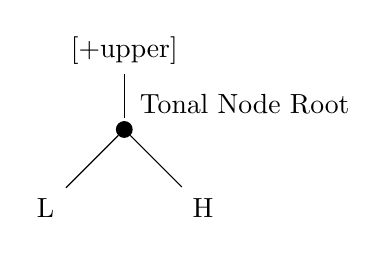
\begin{tikzpicture}[-,shorten >=1pt]
    \tikzstyle{state}=[fill=white,draw=black,text=black,node distance=16mm]

    \node (s1) at (0,0) {[+upper]};
    \node[circle, draw, fill=black, inner sep=2pt,
    label=above right:Tonal Node Root] (s2) at (0,-1) {}; % small filled circle
    \node (T1)  at (-1,-2) {L};
    \node (T2) at (1,-2) {H};

    \draw (s1) -> (s2);
    \draw (s2) -> (T1);
    \draw (s2) -> (T2);
\end{tikzpicture}

    
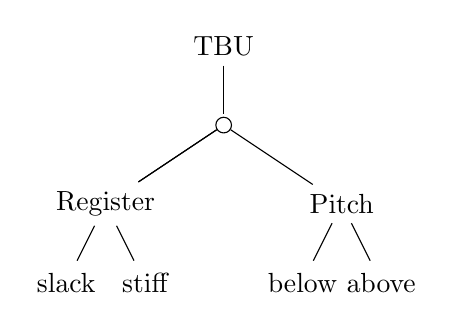
\begin{tikzpicture}[-,shorten >=1pt]
    \tikzstyle{state}=[fill=white,draw=black,text=black,node distance=16mm]

    \node (s1) at (0,0) {TBU};
    \node[circle, draw, fill=white, inner sep=2pt] (s2) at (0,-1) {}; % small filled circle
    \node (T1) at (-1.5,-2) {Register};
    \node (T2) at (1.5,-2) {Pitch};
    \node (p1) at (2,-3) {above};
    \node (p2) at (1,-3) {below};
    \node (r1) at (-2,-3) {slack};
    \node (r2) at (-1,-3) {stiff};
    \draw (s1) -> (s2);
    \draw (s2) -> (T1) -> (r1);
    \draw (s2) -> (T1) -> (r2);
    \draw (s2) -> (T2) -> (p1);
    \draw  (T2) -> (p2);
\end{tikzpicture}

\bibliography{refs.bib}
\bibliographystyle{apalike}
\end{document}